\section{General Infrastructure for Both Web2.0 and Web3.0 Games}


At the most basic level, Carry SDK assists developers in integrating blockchain technology into both traditional and emerging Web3 games. It does not mean building every blockchain game from scratch to completion, which takes a massive amount of time and is a non-standardized process that serves only a limited number of users. From the perspective of efficiency, we want this integration to be a standardized and minimized process.
% \begin{figure}[!htb]
%     \centering
%     \includegraphics[width=1.0\textwidth]{gameinfra.png}
%     \caption{Carry Game Infrastructure provides support for both Web2 and Web3 games in multiple aspects.}
%     \label{fig:gameinfra}
% \end{figure}

Specifically, the proposed infrastructure is composed of three fundamental modules (Asset Management Module, Identity Management Module, and Security Protection Module) and two novel modules (Ad Managment Module and Data Analysis Module). 

\subsection{Asset Management Module}
% We will first need to clarify the core differences between traditional and blockchain games to begin this process. In blockchain games, users control their own game assets, independent of any distinguishable facets of gameplay or mechanics. 

% Carry Game Infrastructure is addressing a critical issue in games: the ownership and control of in-game assets. Traditionally, these assets are merely data on a server, which doesn't guarantee players' permanent control over them. Carry uses blockchain concepts, specifically fungible and non-fungible tokens (FTs \& NFTs), to give players a more reliable way to own and use their assets within games. This shift means that the existence and ownership of an asset aren't solely tied to the game itself but are secured on the blockchain.
The Asset Management Module aims to revolutionize the ownership and tradeability of in-game assets through blockchain technology. By leveraging fungible tokens (FTs) for in-game currencies and non-fungible tokens (NFTs) for unique items, this module ensures true ownership, provenance, and interoperability of assets across different gaming platforms and ecosystems. The core designs are composed of the following three elements:
\begin{itemize}
    \item \textbf{Tokenization:} Utilizing ERC-20 (for FTs) and ERC-721 or ERC-1155 (for NFTs) standards to represent in-game currencies and items on the blockchain.
\item \textbf{Smart Contracts:} Deploying smart contracts to handle the logic for asset creation, ownership transfer, and transactions, ensuring transparency and security.
\item \textbf{Blockchain Layer:} Integration with a blockchain layer (e.g., Ethereum, Binance Smart Chain) for decentralized asset management and to leverage its security protocols.
\end{itemize}

Based on the elements mentioned above, the processes can be summarized as follows: 
\begin{enumerate}
    \item Define asset classes and attributes in smart contracts.
    \item Deploy contracts to the blockchain, generating a unique address for each asset.
    \item Implement game logic to interact with blockchain for asset transactions using Carry SDK.
    \item Use event listeners for real-time updates on asset state changes within the game environment.
\end{enumerate}




\subsection{Identity Management Module}
% In the realm of user identity, traditional games rely on conventional methods like email addresses or social accounts for user registration and login. Carry introduces a new paradigm with Web3, where on-chain addresses become the primary identifier. This approach extends the scope of user interaction beyond just games, as the user's identity and activities are independent of the game server. However, integrating these blockchain elements into games has been challenging for many developers, especially those with extensive experience in traditional game development but limited knowledge of blockchain technology.

% To bridge this gap, Carry has developed a comprehensive Software Development Kit (SDK), making it easier for developers to include blockchain features in their games without needing extensive blockchain expertise. The SDK facilitates the binding of a player's wallet address to their game account, allowing a combination of in-game and blockchain-based accounts. It also enables the tokenization of in-game assets, aligning them with corresponding blockchain contracts. This functionality extends to various asset interactions, such as token generation, minting, and transfers, directly through players' Web3 wallets. Carry's SDK, designed for simplicity and security, provides a range of standardized APIs that developers can use to set up a token-based game economy. It supports various blockchain networks and is compatible with multiple client platforms, enhancing its versatility. 
This module seeks to establish a decentralized identity system that allows game players to use a single, secure, and persistent identity across both Web2 and Web3 gaming platforms. By incorporating Decentralized Identifiers (DID) \cite{reed2020decentralized}, it aims to enhance user privacy, security, and cross-platform interoperability. The core designs are composed of the following three elements:
\begin{itemize}
    \item \textbf{DID Integration:} Utilizing the DID standard for creating verifiable, self-sovereign digital identities tied to blockchain addresses.
\item \textbf{Wallet Binding:} Facilitating the binding of a player’s wallet to their game account, enabling seamless in-game and blockchain interactions.
\item \textbf{SDK Features:} Providing APIs within Carry SDK for easy integration of DIDs, supporting login, authentication, and asset management.
\end{itemize}

\begin{figure}[!htb]
    \centering
    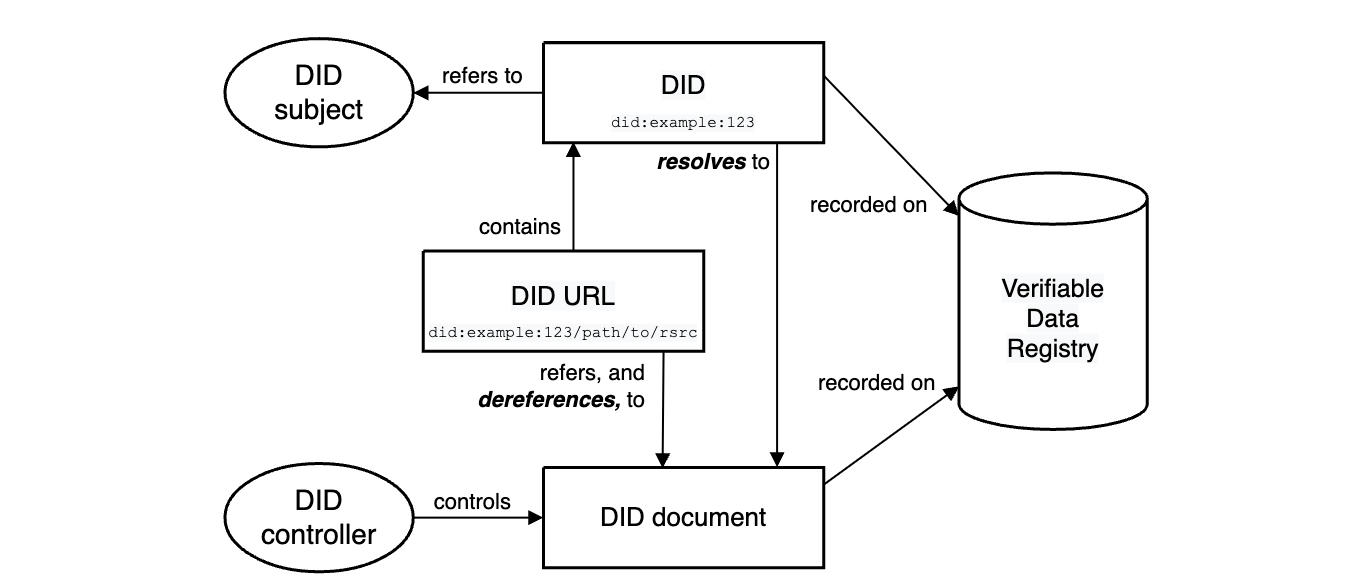
\includegraphics[width=\textwidth]{did.png}
    \caption{Overview of DID architecture and the relationship of the basic components.}
    \label{fig:did}
\end{figure}
We introduce a basic overview of the major components of Decentralized Identifier architecture provided by \href{https://www.w3.org/TR/did-core/}{W3C}, as shown in Figure~\ref{fig:did}. Based on the elements mentioned above, the processes can be summarized as follows: 

\begin{enumerate}
    \item Initialize DID for each user upon registration using Carry SDK.
    \item Bind user's wallet address to their game account, linking in-game and blockchain identities.
    \item Authenticate user actions in-game and on blockchain via digital signatures.
    \item Store and manage user's digital assets and identity securely on-chain.
\end{enumerate}


\subsection{Security Protection Module}
% The SDK also prioritizes security, incorporating features like multi-party computation and private key management mechanisms to ensure the safety of transactions and digital assets within the game environment.
The focus is on ensuring the integrity and security of in-game transactions and digital asset management. By incorporating advanced cryptographic techniques such as multi-party computation (MPC) \cite{feng2023efficient} and zero-knowledge proofs (ZKP) \cite{wang2023zero}, this module aims to protect user assets, maintain privacy, and secure transactions without compromising on user experience.  The core designs are composed of the following three elements:
\begin{itemize}
\item \textbf{Cryptography:} Implementing MPC for secure, distributed private key management and ZKP for transaction validation without revealing sensitive information.
\item \textbf{Smart Contract Security:} Employing security practices like audits and formal verification to ensure smart contract integrity.
\item \textbf{SDK Security:} Ensuring the Carry SDK incorporates the latest security protocols for interaction with blockchain networks, including secure API calls and encryption of sensitive data.
\end{itemize}
 Based on the elements mentioned above, the processes can be summarized as follows: 

\begin{enumerate}
    \item Implement MPC protocols for key management, allowing transactions without exposing private keys.
    \item Use ZKP for transaction validation, ensuring privacy and security.
    \item Conduct regular security audits and update smart contracts and SDK accordingly.
    \item Integrate secure, encrypted communication channels within Carry SDK for asset and identity management.
\end{enumerate}

\subsection{Technical Architecture for Carry SDK}

The above modules collectively provide a robust framework for integrating blockchain technology into gaming, offering a seamless bridge between traditional (Web2) and blockchain-based (Web3) gaming experiences. Through these advancements, Carry Protocol aims to enhance ownership, interoperability, and security for the gaming community. In this section, we demonstrate the detailed technical architecture for Carry SDK, as shown in Figure~\ref{fig:modules}.  

\begin{figure}[!htb]
    \centering
    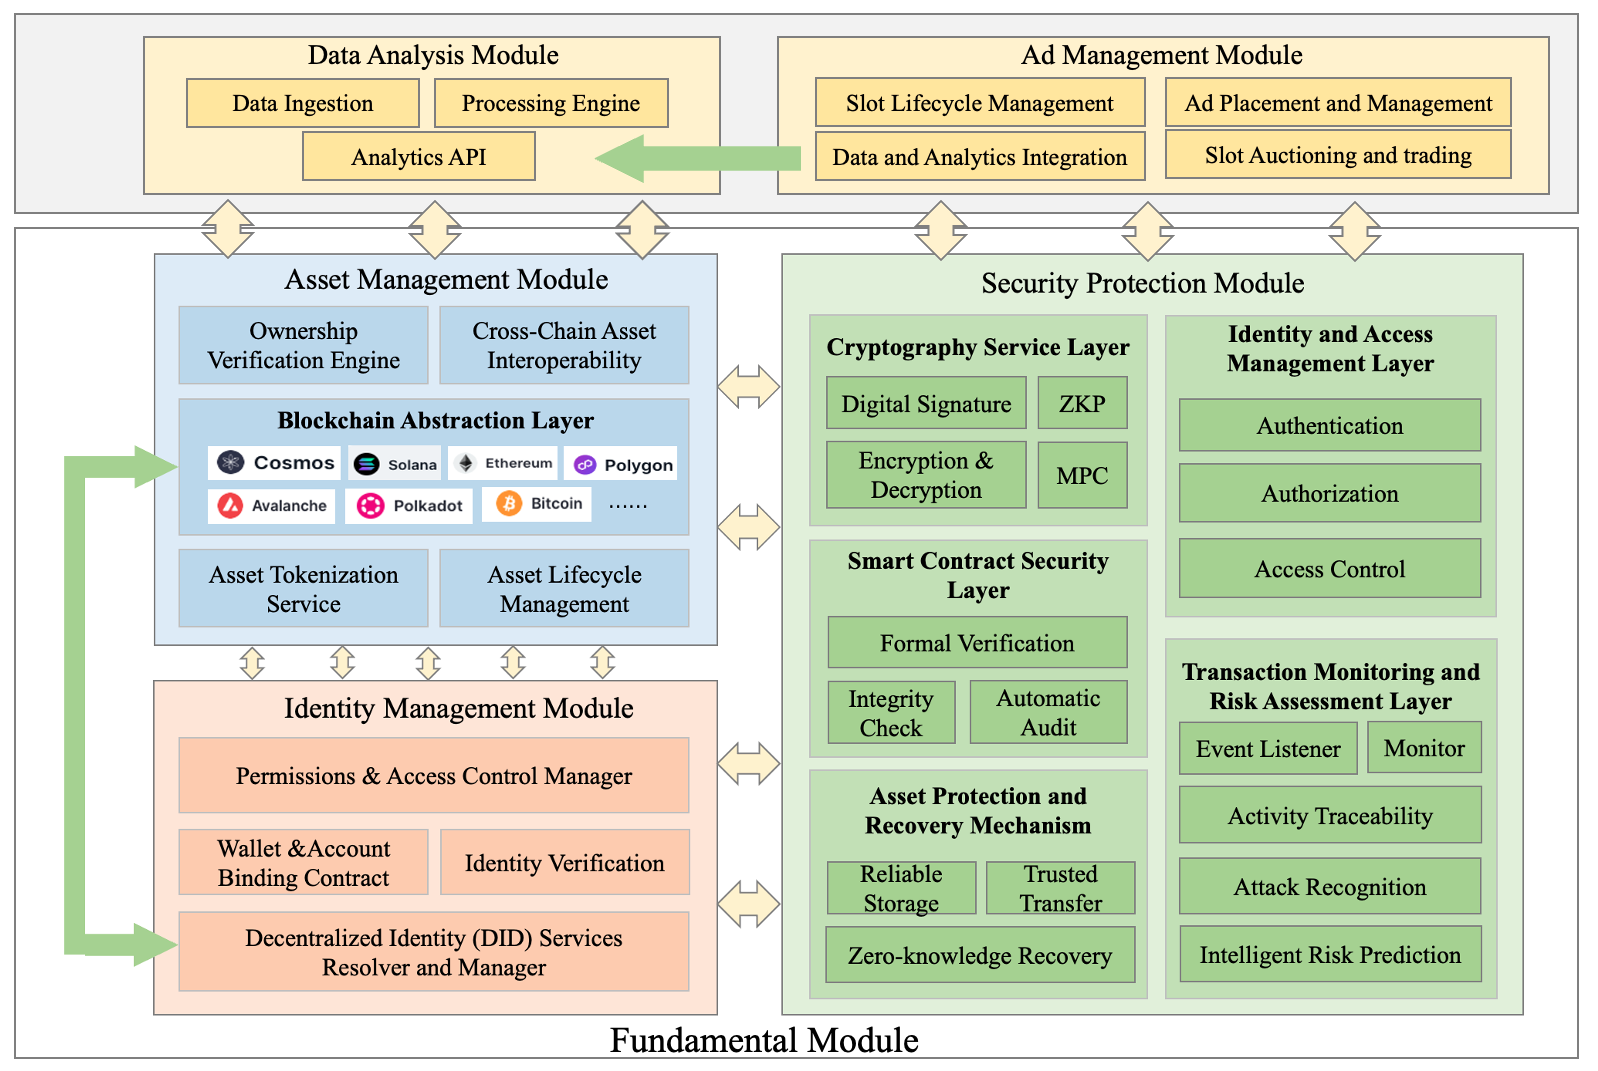
\includegraphics[width=\textwidth]{Technical Architecture Overview of Carry Modules.png}
    \caption{Technical Architecture Overview of Carry SDK Modules.}
    \label{fig:modules}
\end{figure}

\subsubsection{Asset Management Module} 
There are five key components in Asset Management Module. We explain them in a bottom-up manner.
\begin{itemize}
    \item  \textbf{Asset Tokenization Service (ATS):} Converts in-game assets into blockchain tokens. It supports multiple standards (ERC-20, ERC-721, ERC-1155) and manages the lifecycle of tokens including creation, transfer, and destruction.
  \item \textbf{Blockchain Abstraction Layer (BAL):} Serves as the interface between game servers and various blockchain networks, abstracting the complexity of blockchain protocols and offering a unified API for asset transactions.  Interfaces with various blockchains to abstract complexities, providing a unified API for asset transactions across networks like Cosmos, Ethereum, Solona, Polygon, and Binance Smart Chain.
  \item \textbf{Ownership Verification Engine (OVE):} OVE verifies the ownership and authenticity of in-game assets through immutable transactions. This verification process is critical for preventing fraud, duplication, or unauthorized access to assets, thereby ensuring that only rightful owners can initiate transfers or modifications. By providing a trustless mechanism for ownership verification, OVE plays a key role in maintaining a secure and fair gaming environment, where players have full confidence in the value and authenticity of their digital possessions.
  \item \textbf{Cross-Chain Asset Interoperability (CCAI):} Cross-Chain Asset Interoperability (CCAI) addresses one of the key challenges in the blockchain space: enabling assets to move freely and securely across different blockchain networks. CCAI facilitates the trading and exchange of assets between disparate blockchains, enhancing their liquidity and usability. This interoperability is crucial for creating a unified gaming economy where assets from one game or platform can be utilized or traded in another, regardless of the underlying blockchain. By breaking down the barriers between blockchain ecosystems, CCAI enables a more interconnected and fluid digital asset market, where players can leverage the full potential of their in-game assets across the blockchain universe.
\end{itemize}

\subsubsection{Identity Management Module}
There are five key components in Identity Management Module. 
\begin{itemize}
\item \textbf{Decentralized Identity Services:} Decentralized Identity Services form the backbone of the identity management module in Carry Protocol SDK, focusing on managing user identities through decentralized identifiers (DIDs). These services are responsible for the creation, resolution, updating, and revocation of DIDs. By associating a user's DID directly with their game account, it facilitates cross-platform identity verification and usage. DIDs serve as a universal identity marker across different games and platforms, enabling a seamless gaming experience. This system ensures that identities are portable, self-sovereign, and can be verified without reliance on centralized authorities.
\item \textbf{Wallet and Account Binding:} The Wallet and Account Binding component is tasked with securely linking a user's blockchain wallet address to their gaming account. This process is integral for enabling in-game identity verification and asset management through DIDs. By binding the wallet address with the user's DID, it ensures that the user can leverage their blockchain identity within the gaming environment. This linkage is crucial for authenticating transactions and interactions within the game, ensuring that in-game assets and achievements are securely tied to the user's blockchain identity, facilitating a transparent and trustless ecosystem for asset ownership and exchange.
\item \textbf{Identity Verification:} Identity Verification is a critical process within the identity management module that ensures the authenticity of users by leveraging their DIDs. This component utilizes cryptographic methods to verify that actions, transactions, or access requests are genuinely initiated by the rightful owner of the DID. The process involves validating the user's digital signatures and ensuring that the DID associated with a game account matches the blockchain-verified identity. This layer of verification is pivotal for maintaining the integrity of in-game interactions, preventing impersonation, and ensuring that all transactions are securely authenticated.
\item \textbf{Permissions \& Access Control Manager:} The Permissions \& Access Control Manager governs the access rights of users within the gaming environment, based on their DIDs and predefined access policies. This component is essential for defining and enforcing the rules that determine what resources a user can access and what actions they can perform within a game. By leveraging the user's DID for access control, it ensures that only verified and authorized users can interact with sensitive in-game assets or perform certain operations. This mechanism enhances the security of in-game assets and data, preventing unauthorized access and ensuring that game environments remain safe and fair for all participants.
\end{itemize}

\subsubsection{Security Protection Module}
There are five primary components in Security Protection Module. 
\begin{itemize}
    \item \textbf{Cryptography Service Layer (CSL):} The Cryptography Service Layer (CSL) is a foundational component of the security guarantee module, dedicated to providing robust encryption and decryption services. It supports advanced cryptographic technologies, including digital signatures for verifying the integrity and origin of data, as well as Zero-Knowledge Proofs (ZKP) to facilitate transactions and validations without compromising user privacy. By leveraging ZKP and other cryptographic methods, CSL plays a crucial role in ensuring that sensitive user information and transaction details remain confidential, thereby bolstering privacy protection across the blockchain network.
 \item \textbf{Smart Contract Security Framework (SCSF):} The Smart Contract Security Framework (SCSF) focuses on the development and deployment of secure smart contracts, incorporating automated security audits and formal verification processes to identify and rectify common vulnerabilities. This framework ensures that smart contracts, which govern the logic and execution of blockchain transactions, are devoid of loopholes that could lead to unauthorized access or asset theft. By subjecting all smart contracts to rigorous testing and verification, SCSF ensures the integrity of the contracts, safeguarding assets against exploitation and enhancing overall contract security.
 \item \textbf{Identity and Access Management Layer (IAM):} The Identity and Access Management Layer (IAM) manages user identities and access rights, utilizing Decentralized Identity Verification (DID) to enhance security measures. By employing DIDs alongside multi-factor authentication, IAM ensures that only authenticated users can access sensitive operations and data. This approach to identity management not only strengthens security by verifying user identities but also enhances user control over personal information and privacy, ensuring secure and authorized access within the blockchain ecosystem.
 \item \textbf{Transaction Monitoring and Risk Assessment Layer (TMRAS):} The Transaction Monitoring and Risk Assessment Layer (TMRAS) is tasked with the real-time surveillance of blockchain transaction activities. Utilizing machine learning and behavioral analysis techniques, TMRAS assesses the risk levels of transactions, identifying and mitigating potential threats of fraud and theft. This proactive approach to transaction security allows for the timely detection of suspicious activities, ensuring the protection of assets and maintaining the integrity of the blockchain network.
\item \textbf{Asset Protection and Recovery Mechanism (APRM):} The Asset Protection and Recovery Mechanism (APRM) provides a robust defense against unauthorized access and attacks on user assets. Offering solutions for asset recovery in the event of security incidents, APRM ensures the safe storage and transfer of user assets. By implementing measures to quickly restore assets following a breach or loss, APRM plays a critical role in maintaining user trust and confidence in the blockchain's ability to secure digital assets against potential threats and vulnerabilities.
\end{itemize}

\subsubsection{Ad Management Module}
Following the design of core modules in the Carry SDK framework, such as the Asset Management Module, Identity Management Module, and Security Guarantee Module, Carry Protocol introduces a new component: the Ad Management Module. This module is designed to offer an innovative advertising paradigm based on "slots" in blockchain games, integrating advertisements naturally within the game while delivering value to both game developers and advertisers. There are four core components of the Module Framework.
\begin{itemize}
    \item  \textbf{Slot Lifecycle Management:} This component is responsible for overseeing the entire process of a slot's lifecycle, from creation and initialization to the display and updating of advertisements. Game developers can integrate special slots into their games with ease. Once these slots are in place, they can be utilized by developers or players, transforming them into unique digital items. Monitors and updates the status of each slot, ensuring accurate representation within the ecosystem. Intelligently manages the cooperation between different game elements, especially when changes occur.

\item  \textbf{Ad Placement and Management:} Controls the display of advertisement content across various slots, including the addition, removal, and refresh of ads. Once a slot is selected, relevant advertising content is imbued within it. Assesses the impact of displayed advertisements on users or gamers, beginning to generate value.

\item  \textbf{Slot Auctioning and Trading:} Provides a mechanism for the time and positioning of slots to be bid upon and allocated based on market demand and perceived value. Following operations similar to platforms like OpenSea, slots undergo an auction or selection process. Slots are typically leased for a specified duration rather than transferring ownership.

\item  \textbf{Data and Analytics Integration:} Closely integrates with the Data Analysis Module, offering in-depth analysis of ad effectiveness and slot performance. Utilizing the functionalities of the Data Analysis Module, metrics such as click-through rates and conversion rates are analyzed to provide precise advertising strategies for advertisers.
\end{itemize}
By incorporating the Ad Management Module as part of the Carry SDK framework, the Carry Protocol not only redefines the way advertisements are incorporated into video games but also provides new avenues for collaboration between game creators and players. This innovative approach promises to make the gaming experience more engaging while addressing the ownership of digital ad spaces, potentially bringing positive transformations to both the gaming and advertising industries.

\subsubsection{Data Analysis Module}
In addition to the above components, the Data Analysis SDK is structured to seamlessly work within the Carry Protocol ecosystem, enhancing its functionality with dedicated components for comprehensive data analytics. This module is composed of the following three primary components: 
\begin{itemize}
 \item \textbf{Data Ingestion Module:} This component is responsible for capturing both on-chain data and in-game activity data. It employs interfaces that facilitate the streaming of diverse data types into the system, ensuring that data is accurately and efficiently collected for analysis.

 \item \textbf{Processing Engine:} At the core of the SDK is the Processing Engine, which utilizes advanced algorithms for real-time data analysis. This engine processes data from various sources, applying descriptive, predictive, and prescriptive analytics to transform raw data into actionable insights.

 \item \textbf{Analytics API:} The API provides endpoints for accessing the analytics results, allowing developers and advertisers to query specific data points and retrieve insights. This component ensures that the data analysis results are accessible, interpretable, and ready for application.
\end{itemize}


By integrating the Data Analysis Module within the Carry SDK framework, the Carry Protocol ensures that game developers and advertisers have access to a comprehensive suite of tools for data-driven decision-making. This holistic approach not only enhances the gaming experience and economic viability but also enriches the advertisement strategy, making the Carry Protocol a robust foundation for GameFi projects.

\subsubsection{Module Interactions}
% The Carry SDK is meticulously architected to ensure seamless integration and symbiotic relationships among its three core modules: the Identity Management Module, Asset Management Module, and Security Protection Module. At the heart of this integration is the Identity Management Module, which establishes a secure and verifiable framework for user identities using decentralized identifiers (DIDs). This module not only underpins user authentication and access control but also facilitates the secure management and transfer of assets by linking user identities to their digital assets and transactions. The Asset Management Module leverages this secure identity foundation to tokenize in-game assets and manage their lifecycle on the blockchain, ensuring that asset ownership is indisputably tied to the user's identity. This process is further safeguarded by the Security Protection Module, which envelops both the identity and asset management operations in a layer of robust cryptographic services, smart contract integrity checks, and real-time monitoring for transactions and risks. Together, these modules create a comprehensive ecosystem where user identities are securely managed, assets are reliably tokenized and protected, and all interactions within the platform are monitored and secured against potential threats, ensuring a trustworthy and user-centric blockchain gaming experience.
The Carry SDK orchestrates seamless interactions among its five core modules: Identity Management, Asset Management, Security Protection, Ad Management, and Data Analysis. Central to this ecosystem is the Identity Management Module, which authenticates users and links their identities to digital assets and transactions, forming the basis for secure interactions within the SDK. The Asset Management Module utilizes this identity framework to tokenize in-game assets and manage their ownership, ensuring assets are securely linked to users. The Security Protection Module enhances this setup by providing cryptographic security and integrity checks, safeguarding assets and user data against potential threats. Integrating with these foundations, the Ad Management Module leverages user and asset data to place and optimize in-game advertisements, enhancing player experience and advertising value. The Data Analysis Module complements this by analyzing data across modules, offering insights to refine user engagement, asset management, and ad effectiveness.

Together, these modules create a symbiotic environment where secure asset tokenization, personalized advertising, and comprehensive analytics converge to offer a robust and user-centric blockchain gaming experience.
